%%
%%
%%      SECTION: BEAM PATTERN 
%%

%% [intro]
%%________________________________________________________

The NIKA2 beam pattern mainly depends on the IRAM 30\,m telescope and
NIKA2 full (external and internal) optical system characteristics,
whereas the detectors themselves might have an impact at sub-dominant
level (through e.g. time constants or correlated noises).

In this section, we characterize both the main beam, which is
modeled as an elliptical Gaussian, and the full beam pattern including
error beams up to angular scales of 10 arcmin.

%% [Full beam pattern]
%%________________________________________________________
\section{Full beam pattern}% {\color{YellowGreen} Laurence}}
\label{se:fullbeam}

\subsection{Data sets}
\label{se:beammap_set}

The characterization of the IRAM $30\,\rm{m}$ beam pattern observed
through NIKA2 detectors is mainly based on observations of strong
compact sources, such as planets including Uranus, Neptune and Mars,
and bright quasars. We generally use \bm\ scans, which are described
in Sect.~\ref{se:beammaps}.
Most of our beam-related analysis is based on a
set of 18 \bm\ scans acquired during the N2R8 and N2R9 commissioning
campaigns and the N2R12 and N2R14 science pools. Namely, the set
consists of the N2R8 '20170125s243' scan, the N2R9 '20170224s177',
'20170226s415', '20170226s425' and '20170227s84' scans, the N2R12
'20171022s158', '20171023s101', '20171024s105', '20171024s106',
'20171025s41', '20171025s42',  '20171027s49',  '20171028s310',
'20171029s266', '20171030s268' and  '20180117s92' and the N2R14
'20180117s92',  '20180122s82' and  '20180122s309' scans.

This set of \bms\ has been selected from all the available \bms\ at
optimal focus using the baseline selection criteria, as given in
Sect.~\ref{se:data_selection}.



\subsection{Deep beam maps}
\label{se:deep_beam_maps}
We present the two-dimensional distribution of the beam in
Fig.~\ref{fig:beam}. We primary use a map obtained from a combination
of deep observations of strong point sources collected during
\emph{NIKA2-run8} and \emph{run9}. Namely, we use \bm\ scans
of Uranus (scan id '20170125s223' and '20170125s243'),  Neptune
('20170224s177') and the bright quasar 3C84 ('20170226s415'). However,
we checked the stability of our results on single scan maps,
combinations of scans for a single source, and combinations of
shallower scans but spanning a large range of scanning direction. The
data processing includes a mitigation of the correlated noise, which
mainly originates from the atmosphere.  We primarly use a subtraction
of a common mode estimated from the most correlated detectors (the
so-called 'cm one block' method). However, other methods are tested
for assessing the immunity of our results to noise residuals.

\begin{figure}[ht!]
\begin{center}
  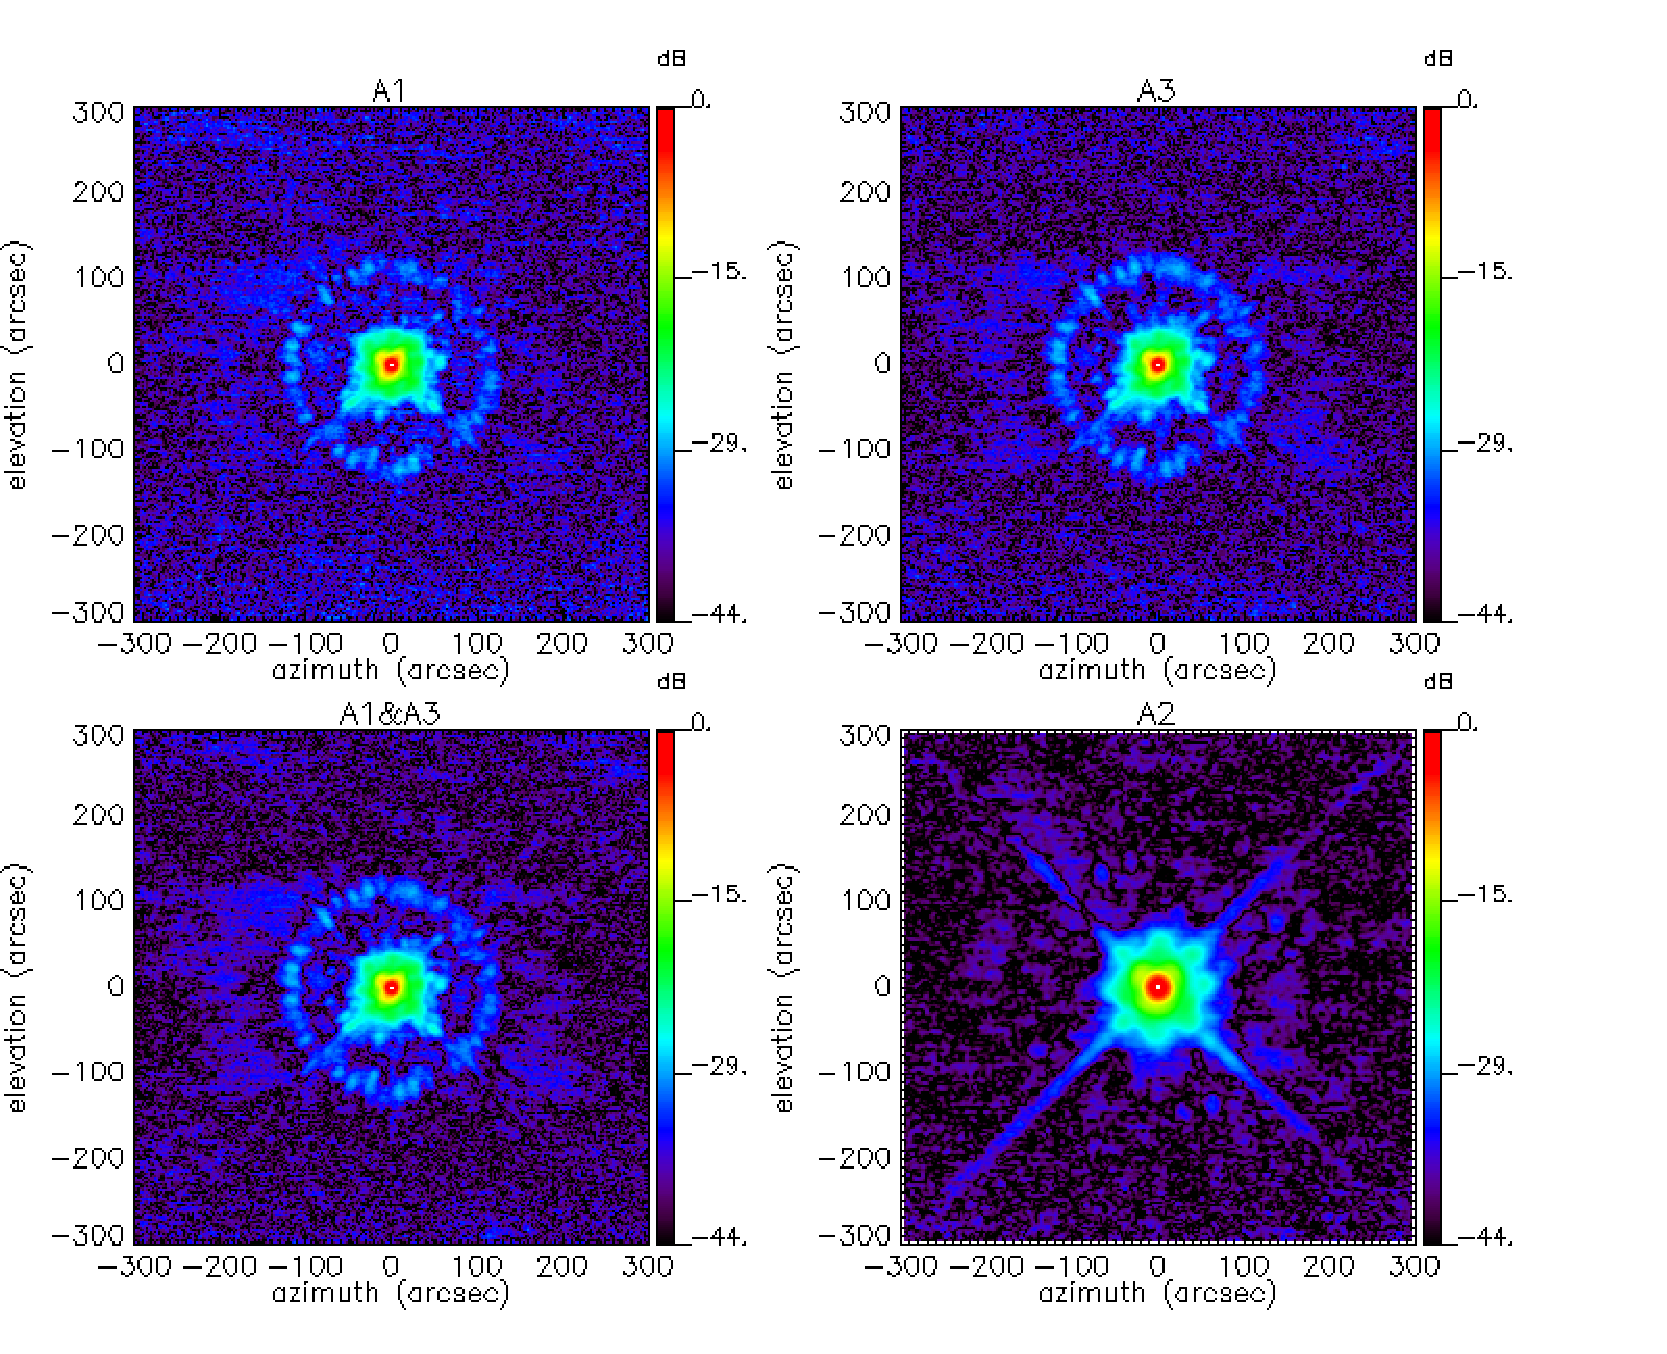
\includegraphics[clip, angle=0, scale=0.4]{Figures/Lobe_map_Combo_v2_dB.pdf}
 \caption[Beam pattern.]{From upper left to lower right, beam maps of array 1 (labeled 'A1'), array 3 ('A3'), the combination of the 1.15mm arrays ('A1$\&$3') and the 2mm array ('A2') are shown in decibel. These maps, which consist of normalized combination of four long OTF scans of bright point sources, are in \new{horizontal} coordinates and cover a sky area which extends over 10 arcmin.}
\label{fig:beam}
\end{center}
\end{figure}


%SAMUEL : diffraction on primary and quadrupod = side lobes. The squarish green feature around the main beam is due to a convolution of the M1/quadrupod diffraction pattern with the pixel transfert function. So from diffraction you have at 1mm: 1st side lobe = 20" diameter, squarish bloc from convolutin with pixel = 60" diameter. And from primary mirror aberrations: 1st error beam due to large scale deformation = 60" diameter, pannel buckling wheel = 120" diameter, 2nd error beam due to frame misalignment (structure below panels) = 220" diamter, 3rd error beam due to individual pannels deformations = 800" diameter. 

The deep NIKA2 beam maps reveal some noticeable features, which are
shown in Fig.~\ref{fig:features}. Ranging from strong and/or extended to
weak and/or spiky, they include:
\begin{itemize}
\item[(1)] \sam{the main beam and the underlying first error
  beam, which is due to the large scale deformations of the primary
  mirror, and the first side lobes. \sam{The latter include 
  the 20" diameter first side lobe and the 60" diameter (squarish)
  side lobe, which is due to the convolution of the primary mirror and quadrupod
  diffraction pattern with the pixel transfert function}; }.
  %The four symmetrical spokes of the error beam as shown by
  %yellow arrows in the A2 panel, are expected from ZEMAX
  %simulations;
\item[(2)] \sam{the diffraction ring by panel buckling of the primary mirror, as shown with
  a red circle in the A1 panel};
\item[(3)] \sam{the side lobes shown with green
  diagonal lines in the A2 panel are due to diffraction on the
  quadrupod holding the secondary mirror of the telescope, as expected
  from ZEMAX simulations};  
\item[(4)] spikes of not fully understood origin pointed with yellow
  arrows. The ones that are along the vertical and
  horizontal axes are reproduced by ZEMAX simulation but at a 
  shallower level, whereas the ones shown in the A3 panel in the
  diagonal directions may be due to the external calibrator,
  \new{which was installed in the vertex tunnel
    for tests during these observations. The origin of the asymetry on
    the 1mm arrays is unknown but most probably due to internal optics
    aberrations};
\item[(5)] shallow spikes of unknown origin, which are circled by pink
  ellipses. The multiple images on the combined deep beam map indicate
  a rotation of these spikes with the observing elevation, which in
  turn point to diffraction related issue or a ghost image that are
  formed inside the cryostat.
\end{itemize}

\begin{figure}[ht!]
\begin{center}
  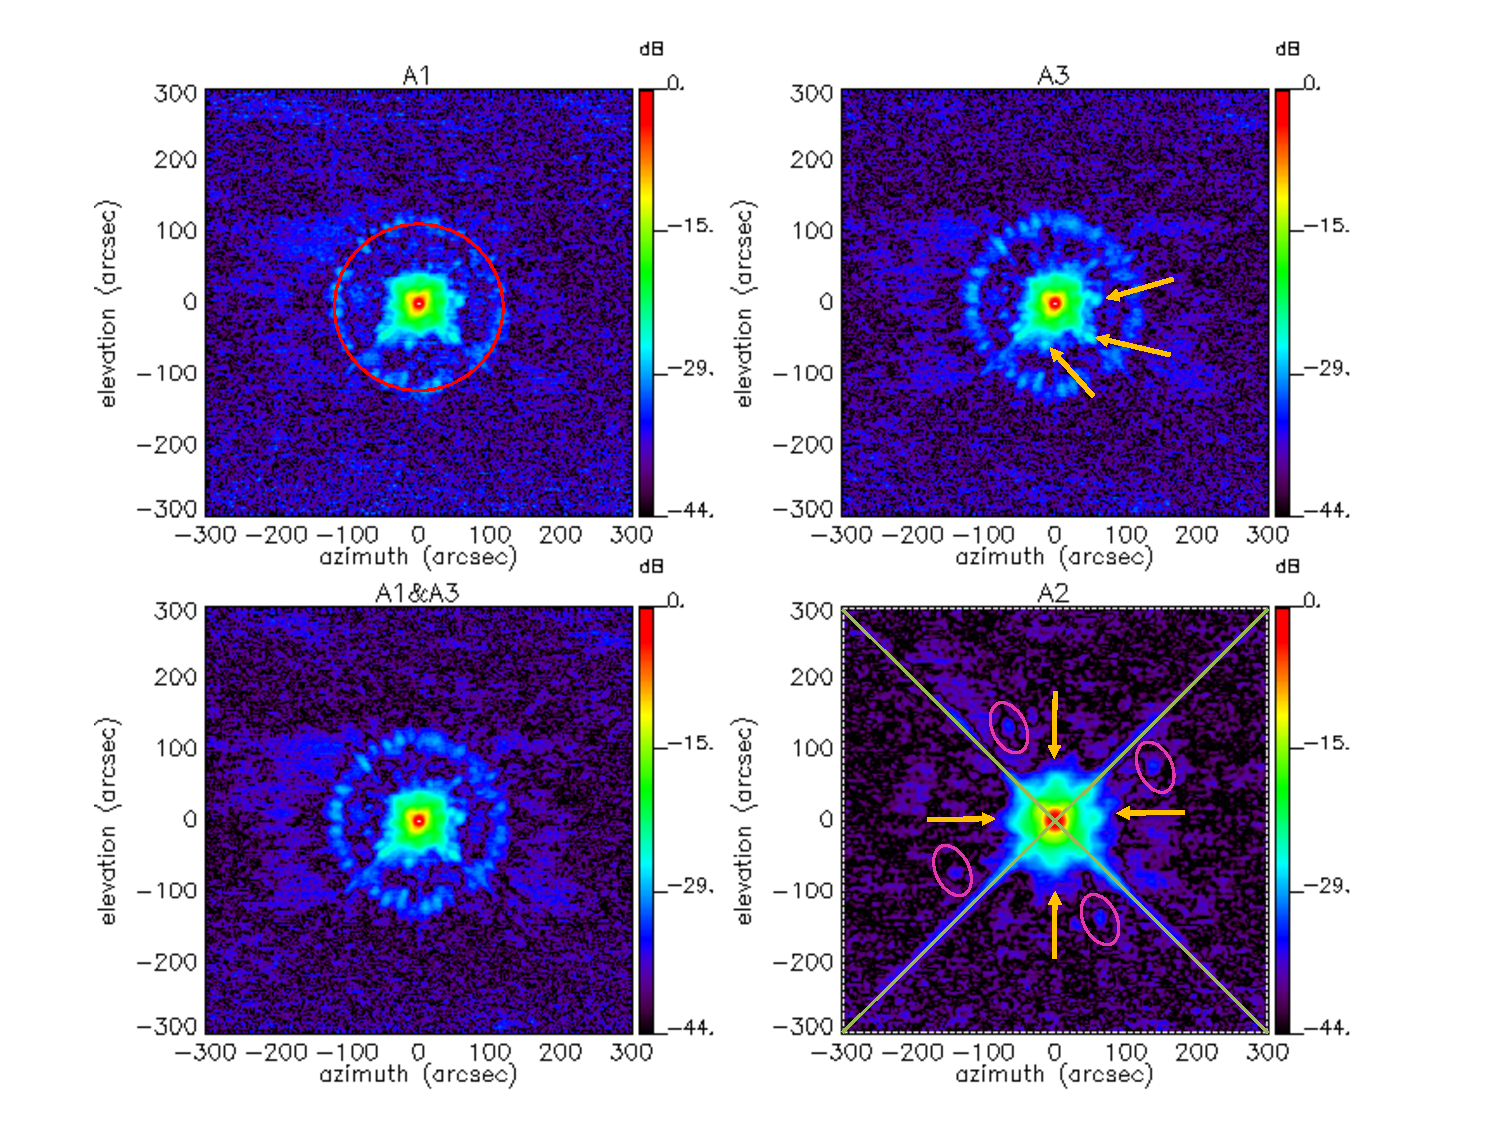
\includegraphics[clip, angle=0, scale=0.4]{Figures/Beams_features.pdf}
\caption[Noticeable features of NIKA2 beam pattern.]{\new{Same maps as in
  Fig.~\ref{fig:beam} with some noticeable features.} Red circle in the
  A1 map (upper left panel): diffraction ring seen in 1-mm maps
  (the spokes are presumably caused by radial and azimuthal panel buckling (cf. Fig.4 in Greve et
  al. 2010)); Orthogonal green lines in the A2 map (lower right panel): diffraction
  pattern caused by quadrupod secondary support structure (prominently
  seen in A2 map); Yellow arrows in the A3 map (upper right panel):
  pattern of 3 spikes seen in 1mm maps of unknown origin; Yellow
  arrows in A2 map (lower right panel): four symmetrical spikes of the
  first sidelobes; Pink ellipses: 4 spikes seen in A2 maps.}
\label{fig:features}
\end{center}
\end{figure}


To gain a first impression of the structure of the IRAM 30-m beam as
seen with NIKA2, we use radial cuts to put in evidence the relative level of
the main beam, the first side lobes and error beam and other features seen in the 2D
beam pattern. NIKA2 full beam is shown in the left
panels of Fig.~\ref{fig:beam_structure_example} by means of two
orthogonal cuts through Uranus from a high quality map obtained on
2017 January 25th in excellent observing conditions
(low opacity $\tau_{225}=0.08$ and elevation $46^{\circ}$).


\begin{figure}[ht!]
  \begin{center}
    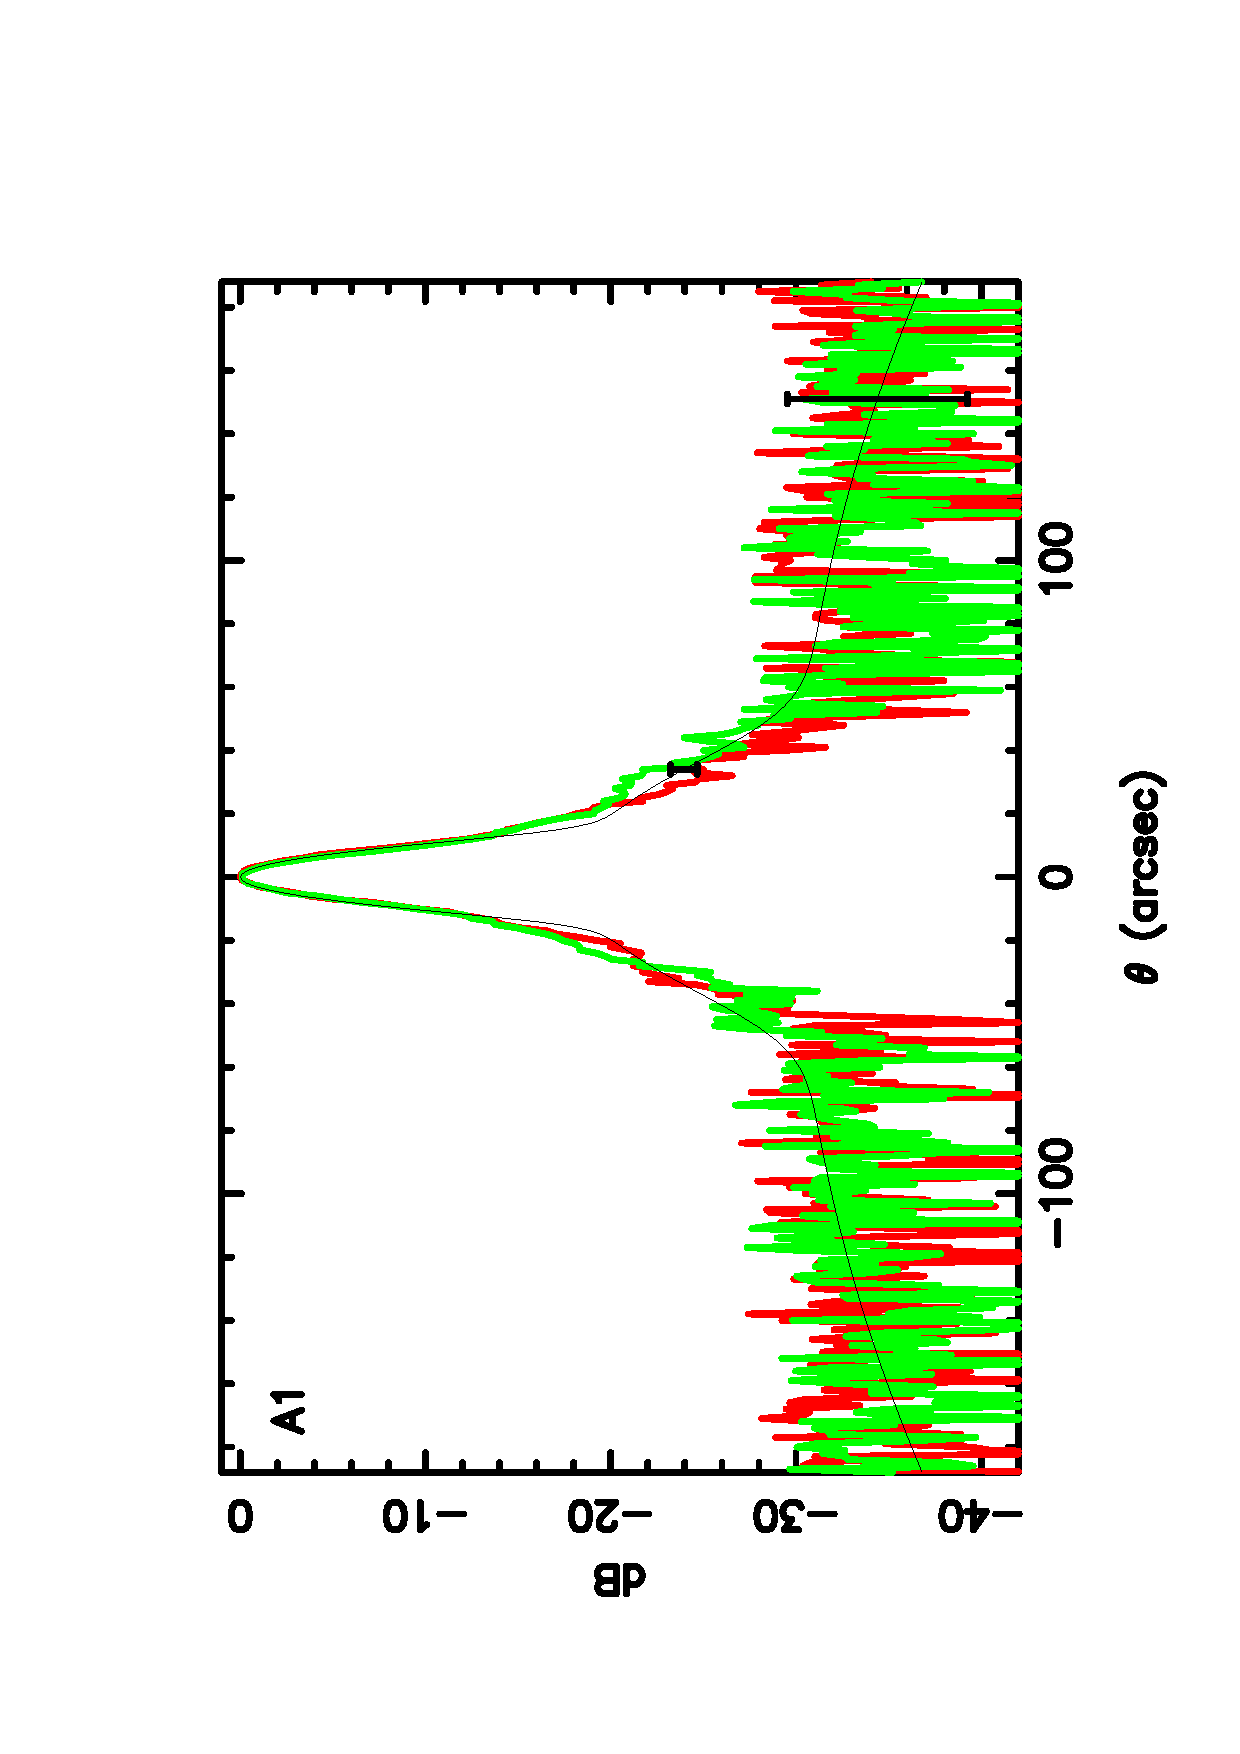
\includegraphics[clip=true, width=0.39\textwidth]{Figures/Array_A1_dB.pdf}
    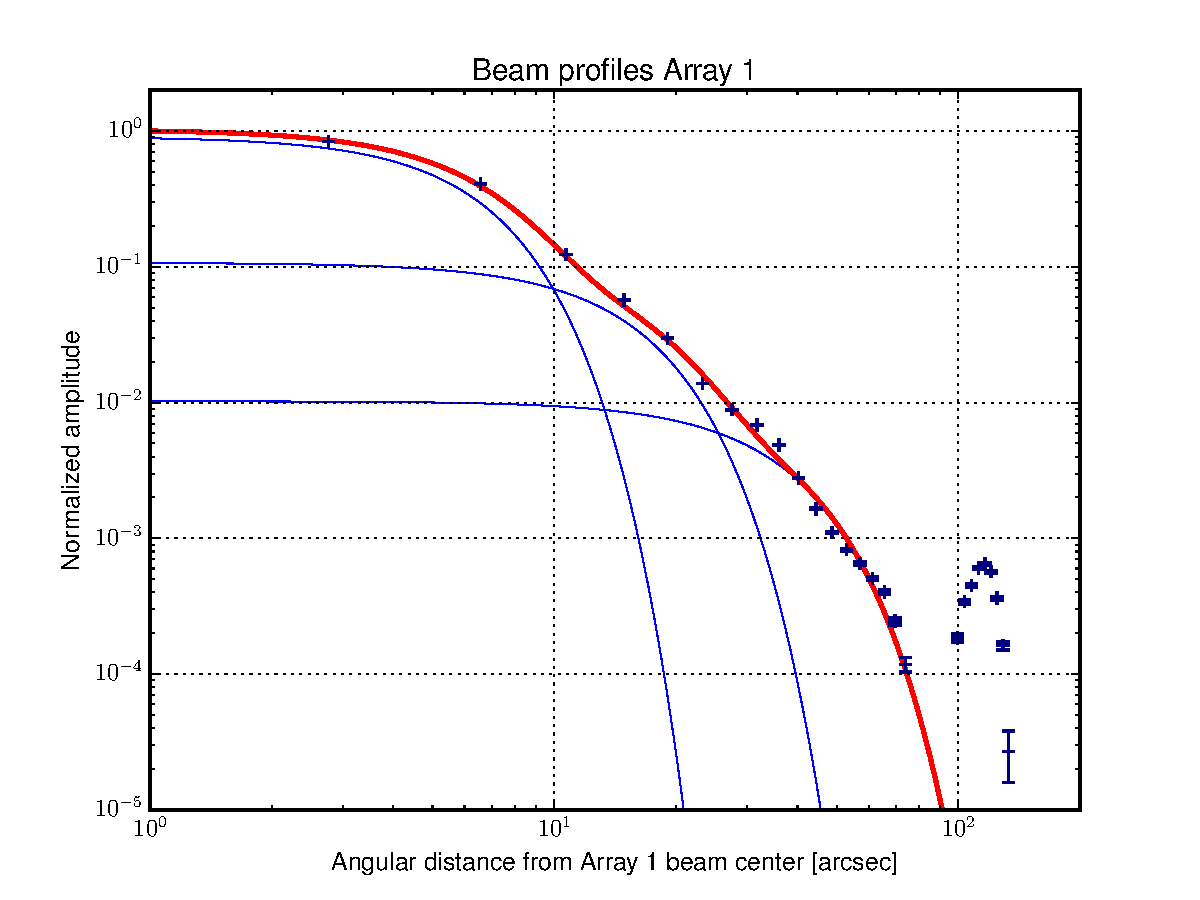
\includegraphics[clip=true, trim={-0.5cm, -0.65cm, 0, 0}, width=0.44\textwidth]{Figures/Beam_profiles_A1_FR.pdf}
    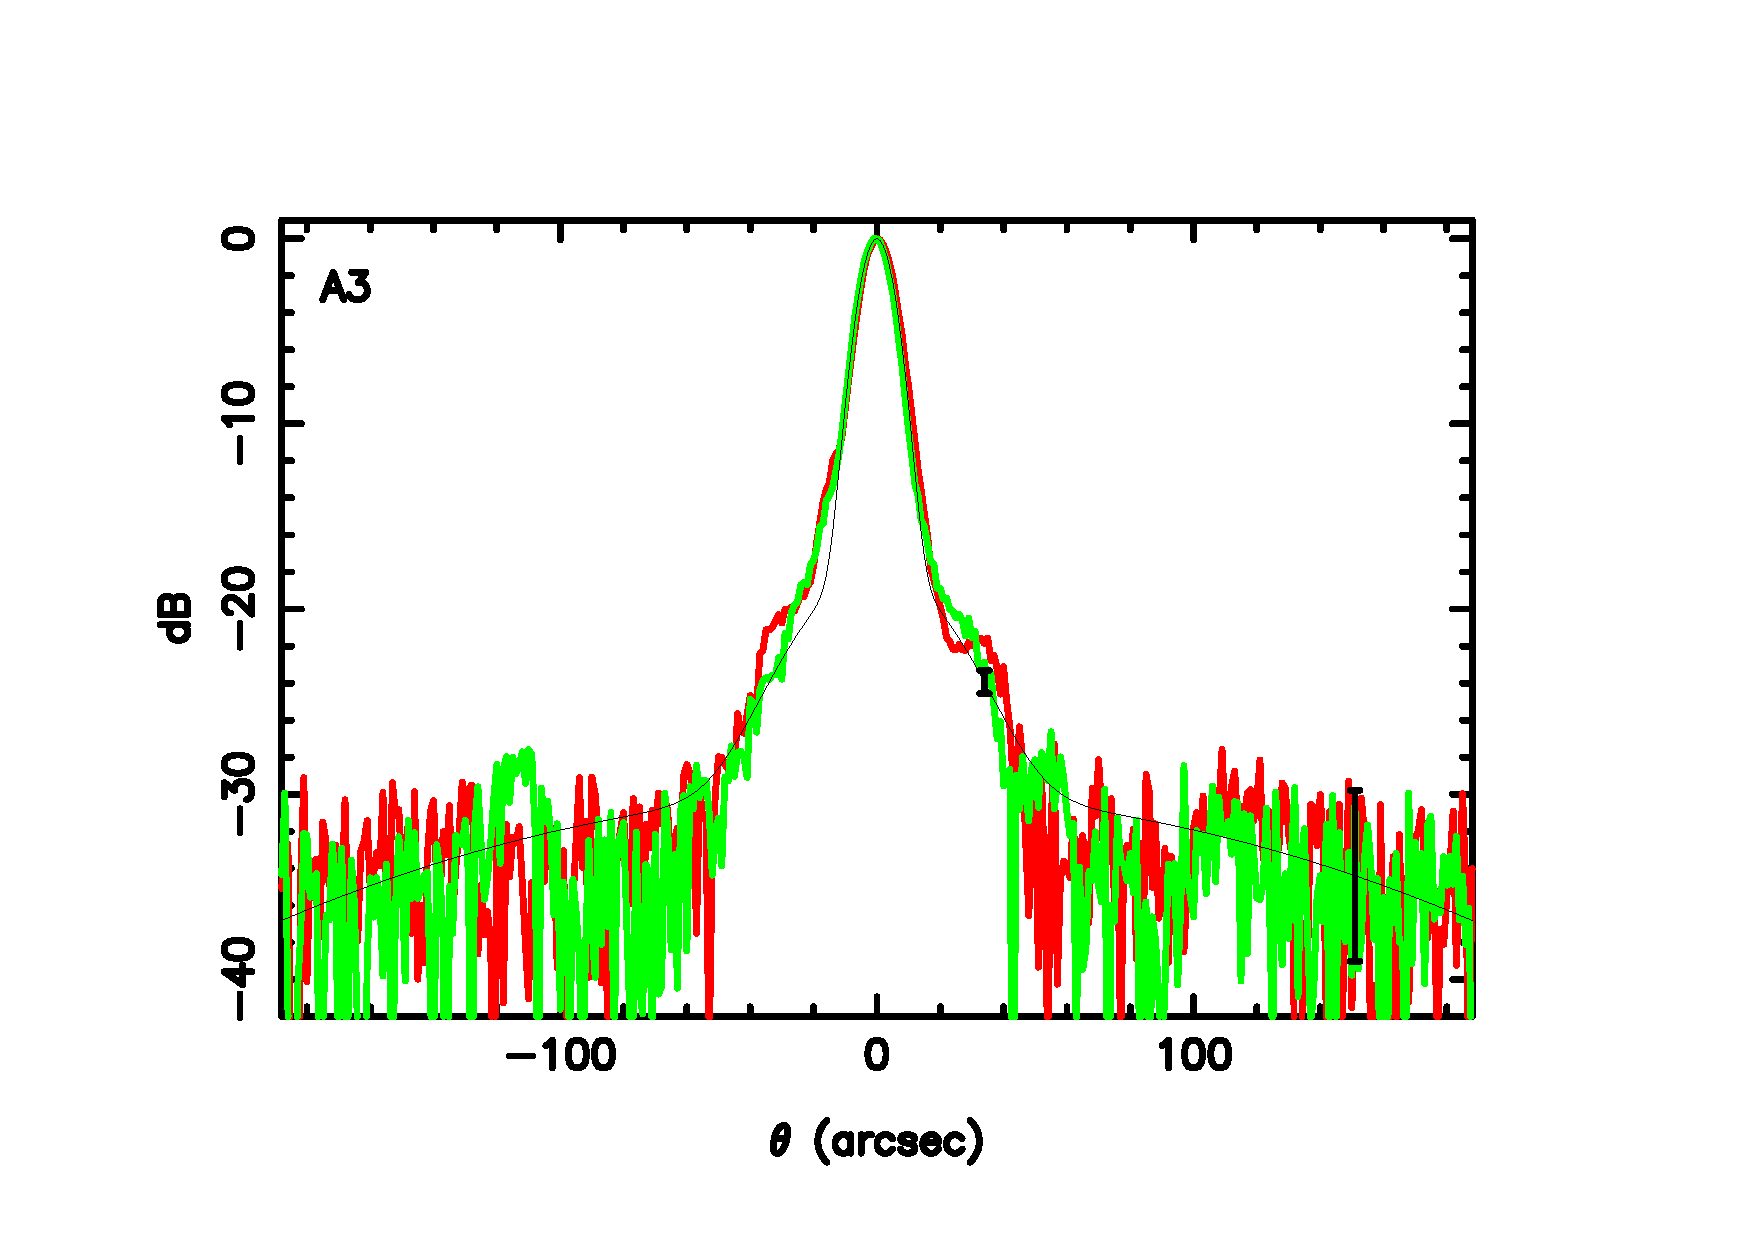
\includegraphics[clip=true, width=0.39\textwidth]{Figures/Array_A3_dB.pdf}
    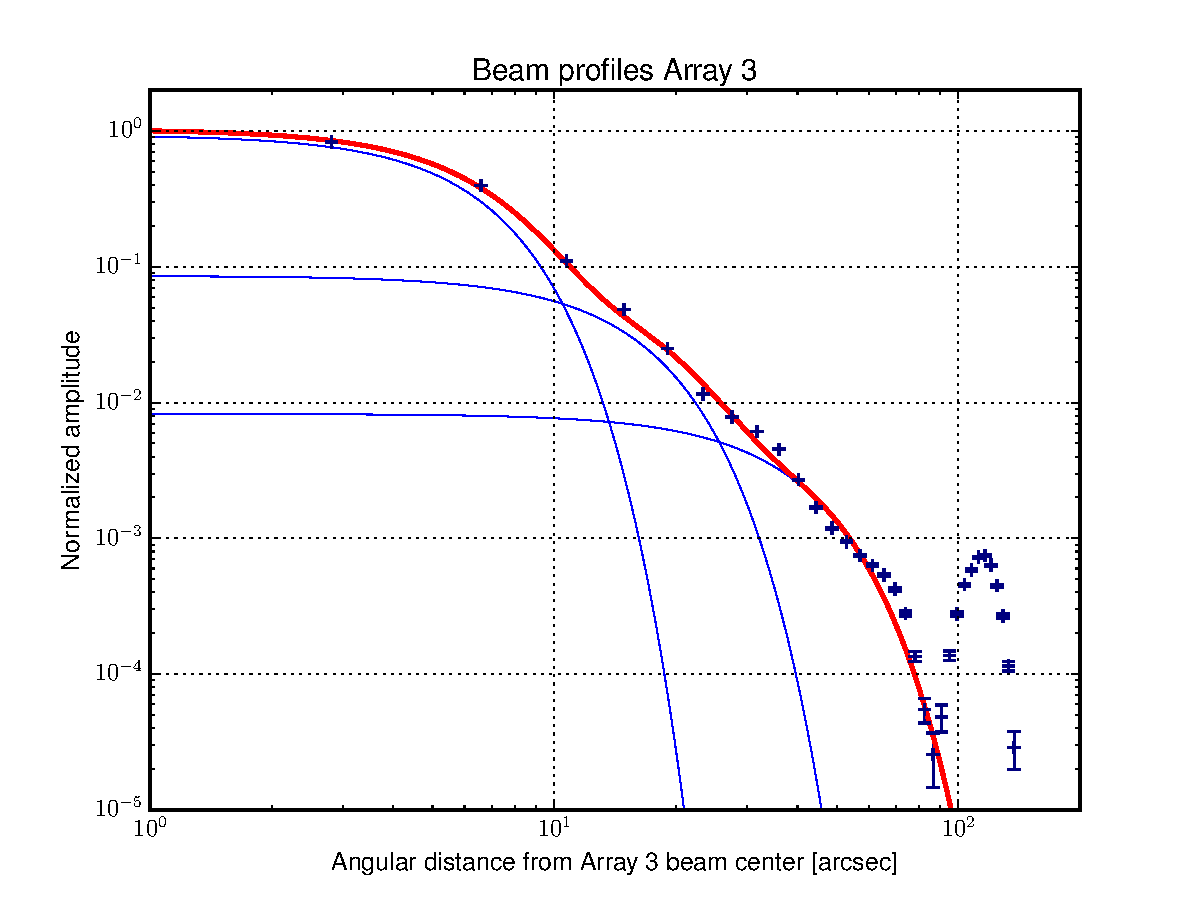
\includegraphics[clip=true, trim={-0.5cm, -0.65cm, 0, 0}, width=0.44\textwidth]{Figures/Beam_profiles_A3_FR.pdf}
    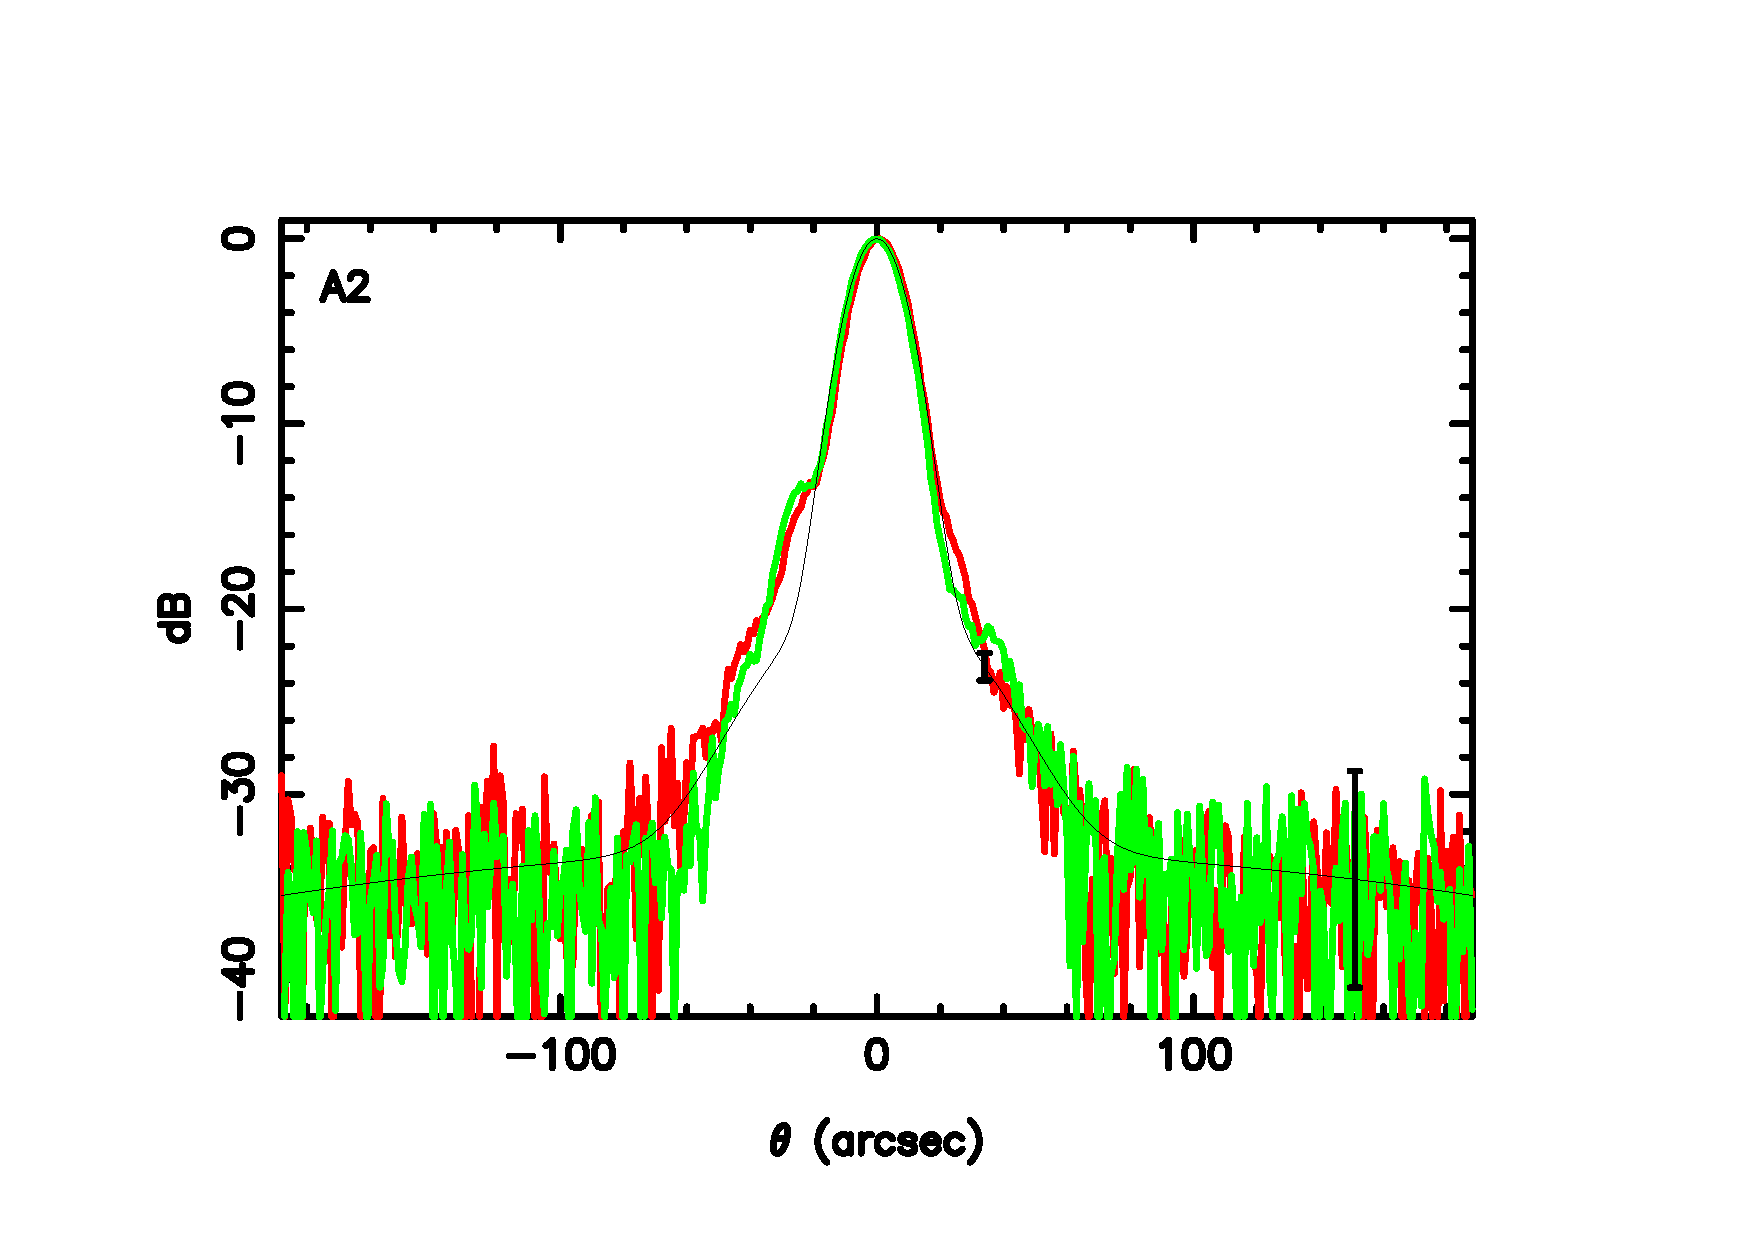
\includegraphics[clip=true, width=0.39\textwidth]{Figures/Array_A2_dB.pdf}
    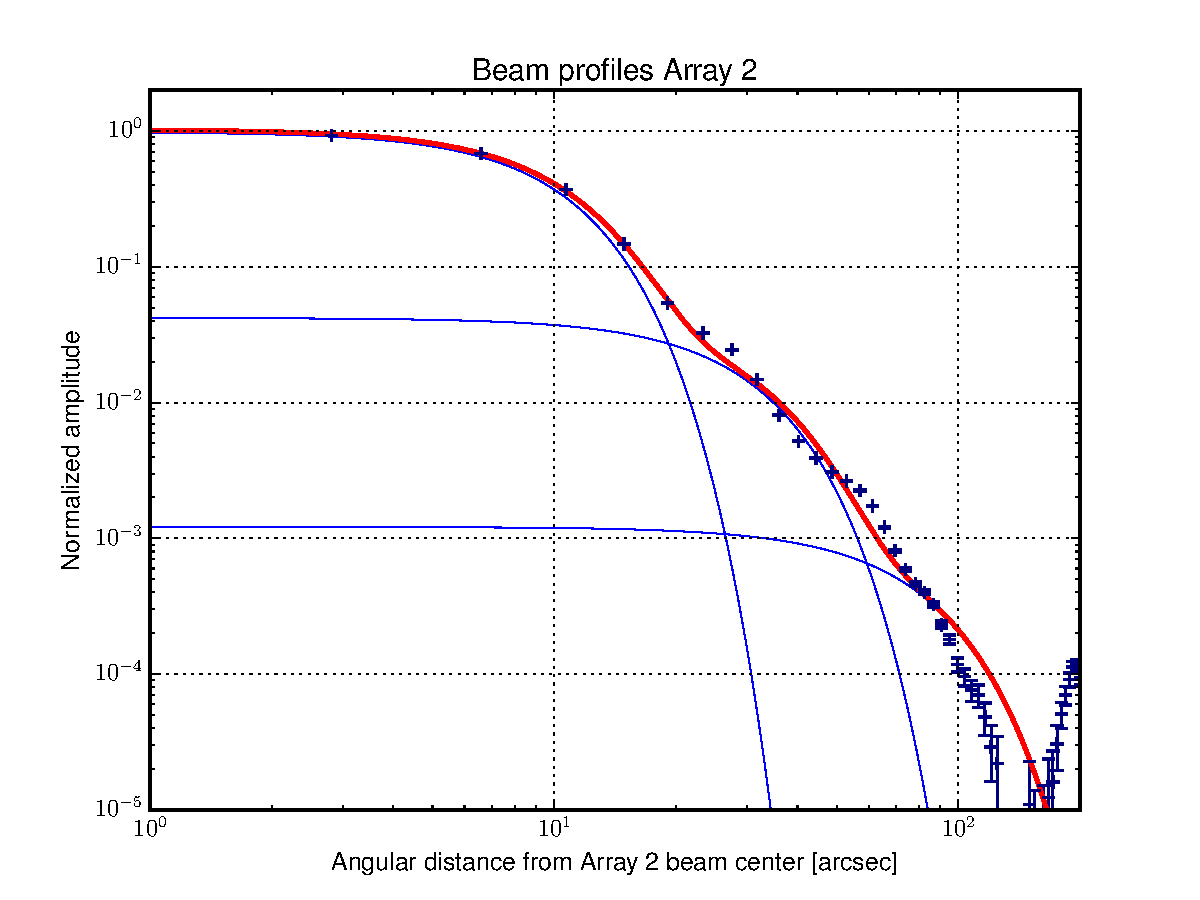
\includegraphics[clip=true, trim={-0.5cm, -0.65cm, 0, 0}, width=0.44\textwidth]{Figures/Beam_profiles_A2_FR.pdf}
    \caption[Beam structure]{\emph{Left column:} Two orthogonal cuts through the
      beam are shown in red and green and a best fit model made of three
      Gaussians is superimposed in black.
      These cuts were obtained from a high quality map of Uranus on 2017
      January 25th at $19:19:58$ UT hours. The main beam starts to depart from the first Gaussian
      at -12dB. \emph{Right column:} Example of beam radial profile
      estimated on the same map of Uranus. The best-fitting curve is shown
      in red using a three Gaussian model.   
    }
    \label{fig:beam_structure_example}
    %\label{fig:beam_profiles_3G}
  \end{center}
\end{figure}

A model made of three Gaussians centered on the source peak was best
fitted {\it by hand} to these cuts.
%the parameters are reported in Table \ref{tab:3gauss} [PEUT-ETRE
%AVANTAGEUSEMENT REPLACED PAR VALEURS DE FLORIAN].
We observe that the main beam starts to depart from the first
Gaussian at the level of about -12dB for the three arrays.
We note that for the instrument EMIR on the radiotelescope,
this departure is about -20dB~\cite{Kramer2013}. However, this
discrepancy between a feedhorn-based experiment and a bare pixels one
is expected since the main effect of the feedhorns is to lower the
side lobes of the Airy diffraction pattern.
%The precise characterization of the full beam structure is discussed
%in Sect.~\ref{se:fullbeam_prof}.  

%From parameters in Table \ref{tab:3gauss}, one can estimate that
%the source incident power is split about equally between the main beam
%and the error beam at 1mm, and these fractions are 70\% and 30\% at 2mm, respectively.
%This modelling uses the central
%region   $180'' \times 180''$ in size with a uniform noise rms from
%a larger area of 8' x 5' on the sky scanned with the arrays. It is expected
%that the error beam extend beyond these limits.


%\begin{table}
%\centering 
%\caption[]{Model parameters of the three Gaussian beam.}
%\begin{tabular}{|l|l|l|l|l|l|l|}
%\hline
%               & \multicolumn{3}{c|}{A1 and A3} & \multicolumn{3}{c|}{A2}  \\
%\hline
%fwhm      & $11.25''$ & $45''$  & $250''$ & $17.75''$ & $56''$  & $420''$ \\
%amplitude & 0.984     & 0.015   & 0.0005   &  0.9875   & 0.011   &  0.0005\\
%\hline
%\end{tabular}
%\label{tab:3gauss}
%\end{table}


\subsection{Beam profile}
\label{se:fullbeam_prof}

\sam{We further quantify the respective level of the axi-symmetrical
  features of the beam pattern in evaluating the beam radial profile}
 $B(r)$, which is the normalised radial brightness profile,
where $r$ is the radius from the beam center.
%is the azimuthal average of the beam map around the
%main beam center.
Although the profile cannot represent the sub-dominant non-axisymmetrical
features, which are seen in the beam pattern and discussed in
Sect.~\ref{se:deep_beam_maps} (quadrupod diffraction pattern, spikes), it provides us with a useful
representation of the internal and central parts of the beam (about up to
$100''$). We determine a beam profile from a beam map in centering to
the fitted value of the main beam center and in forming the
weighted average of the map pixels in annular rings.

We model the beam profile $B(r)$ as a three-Gaussian function defined as:
\begin{equation}
  B(r) = \sum_{i=1}^{3} \mathcal{A}_i G_i(r) + \mathcal{B}_0,
  \label{eq:3gauss}
\end{equation}

where $\mathcal{A}_i$ is the amplitude of the Gaussian $i$ for $i \in {1, 2, 3}$ and
$\mathcal{B}_0$ a pedestal level accounting for the residual noise
level in the map.
An example of the beam profile from a beam map acquired during {\emph N2R8} (scan ID:
20170125s223), as well as the best-fit 3-Gaussian model, is shown in
the right panels of Fig.~\ref{fig:beam_structure_example}.


%%%%%%%%%%%%%%%%%%%%%%%%%%%%%%%%%%%%%%%%%%%%%%%%%%%%%%%%%%%%%%%%%
% Stability of the beam pattern
\begin{figure}[ht!]
  \centering
   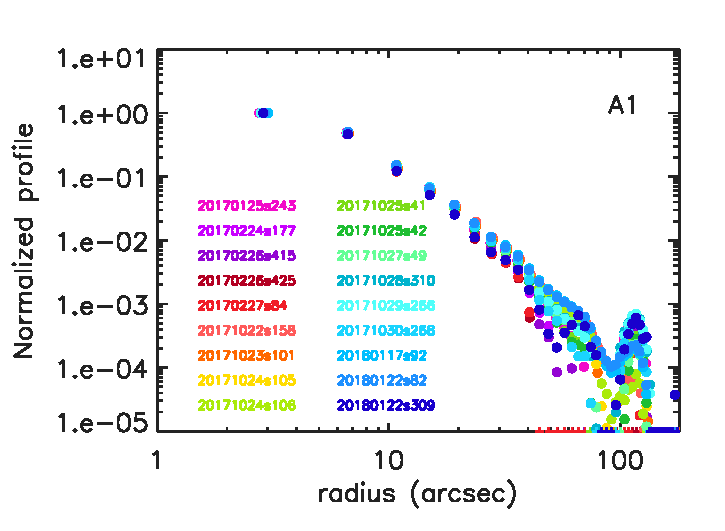
\includegraphics[clip, width=0.42\textwidth]{Figures/Beams/plot_profiles_a1.pdf}
   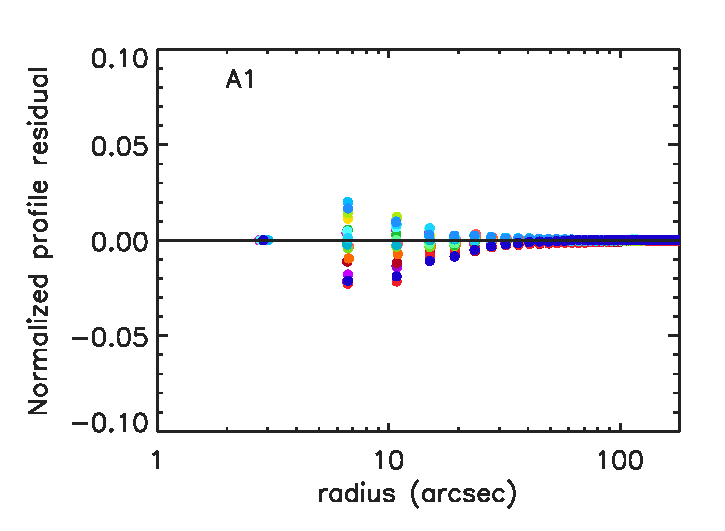
\includegraphics[clip, width=0.42\textwidth]{Figures/Beams/plot_profile_diff_wrt_median_a1.pdf}
   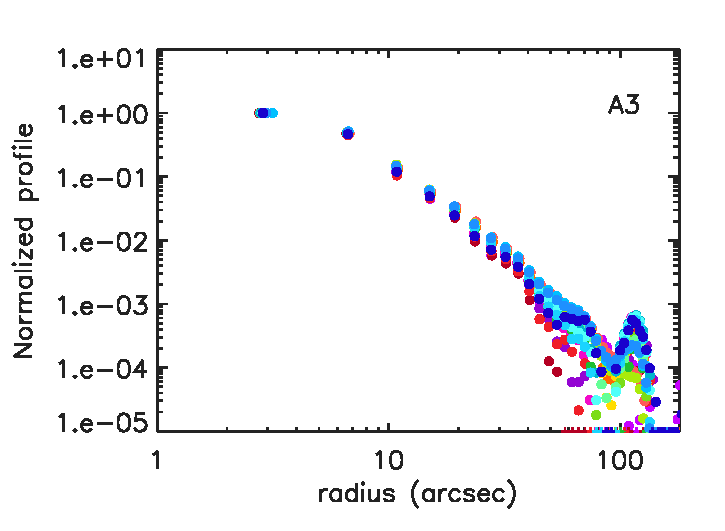
\includegraphics[clip, width=0.42\textwidth]{Figures/Beams/plot_profiles_a3.pdf}
   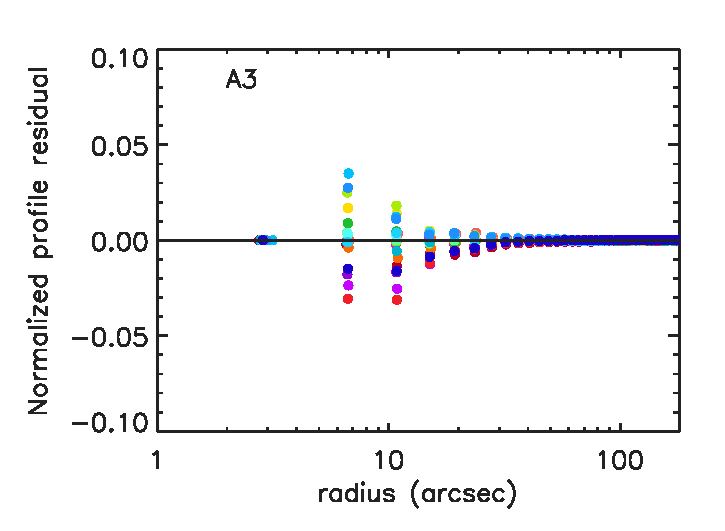
\includegraphics[clip, width=0.42\textwidth]{Figures/Beams/plot_profile_diff_wrt_median_a3.pdf}
   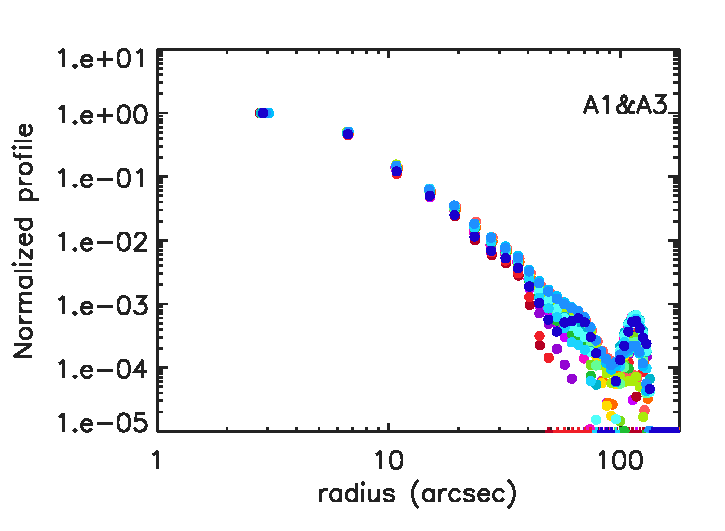
\includegraphics[clip, width=0.42\textwidth]{Figures/Beams/plot_profiles_1mm.pdf}
   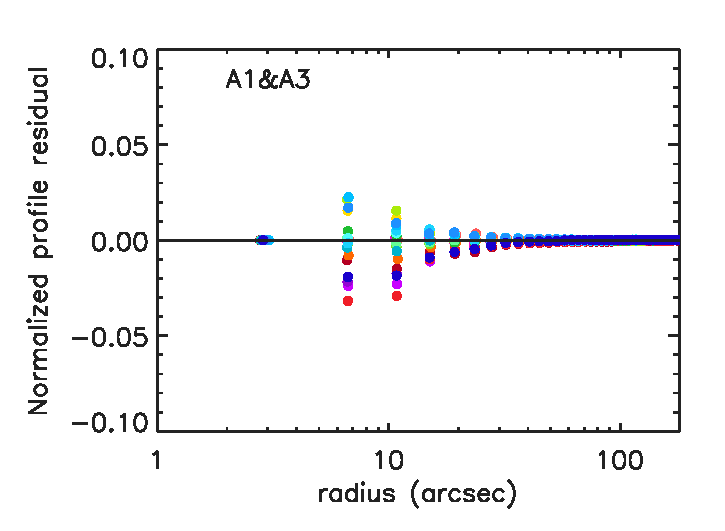
\includegraphics[clip, width=0.42\textwidth]{Figures/Beams/plot_profile_diff_wrt_median_1mm.pdf}
   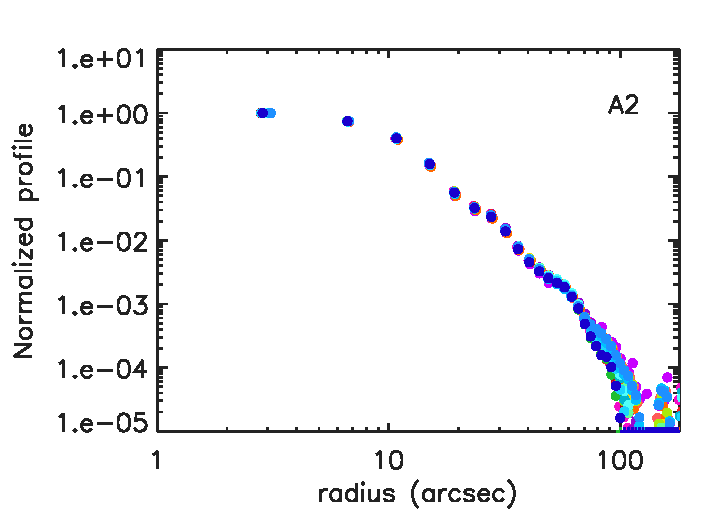
\includegraphics[clip, width=0.42\textwidth]{Figures/Beams/plot_profiles_a2.pdf}
   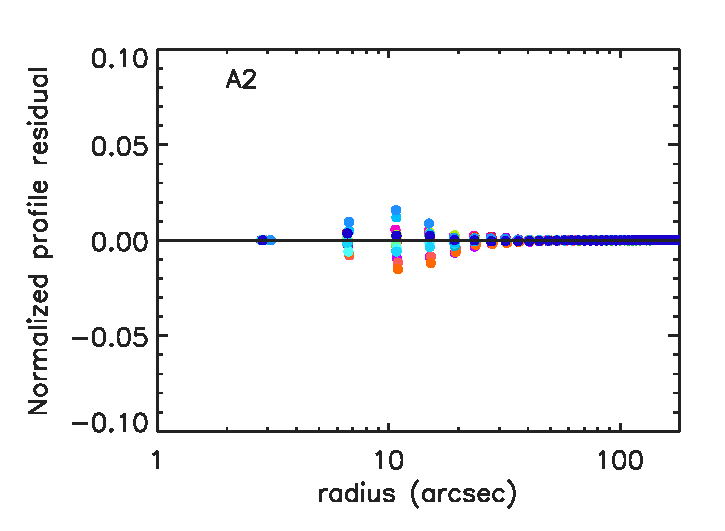
\includegraphics[clip, width=0.42\textwidth]{Figures/Beams/plot_profile_diff_wrt_median_a2.pdf}
  \caption[Stability of the beam profile]{Beam radial profiles as a
    function of the radius from the peak for a series of 18
    \bm\ scans acquired during the N2R8 and N2R9 calibration campaigns and
    during the N2R12 and N2R14 science pools. Left column plots: 
    beam profiles normalised to the maximum value; Right column plots:
    difference w.r.t. the median normalised profile. The radial
    profile shapes are stable at better than $5\%$ 
    against observing conditions.}
  \label{fig:beam_prof}
\end{figure}
We checked the stability of the beam against various observing
conditions (source intensity, weather condition, focus optimisation) by
comparing the beam profiles of the \bm\ set, as described in
Sect.~\ref{se:beammap_set}. The 18 beam profiles and their difference
w.r.t. the median beam profile are shown in Fig.~\ref{fig:beam_prof}.
The variations of the normalised radial profiles are below $5\%$ at
$1\,\rm{mm}$ and below $2\%$ at $2\,\rm{mm}$. 

We further fit the three-Gaussian model of Eq.~\ref{eq:3gauss} to each
profile and gather the average best-fitting amplitudes with respect to
the peak amplitude and FWHM in Table~\ref{tab:mean_3gauss_fit}. The
errors are evaluated as the standard deviation of the best-fitting
parameter values of the 18 \bm\ scans, and thus do not account for the
correlation between parameters. These values are given to gain insight
of the axisymmetrical pattern of the beam, but are not further used for
the calibration. 


% AVERAGE 3-GAUSSIAN FIT
\begin{table}[th]
  \begin{center}
    \begin{tabular}{|c|c|c|c|c|c|c|}
      \hline
      & \multicolumn{6}{|c|}{3-Gaussian profile parameters}  \\\cline{1-7}
      Arrays       & Amp 1 & Amp 2 & Amp 3 & FWHM 1 & FWHM 2 & FWHM 3 \\
      \hline\hline
      A1        &  $0.89 \pm 0.01$   &  $0.08 \pm 0.02$  & $5 \times 10^{-3} \pm 2 \times 10^{-3}$  &  $11.0 \pm 0.2 $ & $29 \pm 2 $  & $65 \pm 15 $ \\  
      A3        &  $0.90 \pm 0.01$   &  $0.07 \pm 0.01$  & $4 \times 10^{-3} \pm 2 \times 10^{-3}$  &  $11.0 \pm 0.2 $ & $30 \pm 3 $  & $72 \pm 23 $ \\  
      1mm       &  $0.90 \pm 0.01$   &  $0.07 \pm 0.01$  & $4 \times 10^{-3} \pm 2 \times 10^{-3}$  &  $11.0 \pm 0.2 $ & $29 \pm 2 $  & $70 \pm 15 $ \\  
      2mm       &  $0.96 \pm 0.01$   &  $0.3 \pm 0.3$    & $1 \times 10^{-3} \pm 0.3$ &  $17.5 \pm 0.1 $ & $63 \pm 10 $ & $65 \pm 12 $ \\  
      \hline\hline
    \end{tabular}
    \caption[Average 3-Gaussian beam profile parameters]{Average
      3-Gaussian beam profile parameters. The FWHMs are given in arcseconds.}
    \label{tab:mean_3gauss_fit}
  \end{center}
\end{table}
